
%\begin{table}
%	\begin{tabular}{ C{1.5cm} | C{0.7cm} C{2cm} C{1.5cm} C{1cm} C{1cm} C{1cm} C{2cm} C{2cm} | C{2cm} }
%		& age & MyasteniaGravis & arthritis & c3level & c4level & hematological & skinrash & sledai2kInferred & SDI \\
%		\hline
%		Visit 0 & 44.23 & 0 & 1 & 119 & 9 & 0 & 0 & 12.0 & 0 \\
%		Visit 1 & 44.63 & 0 & 0 & 96  & 7 & 0 & 0 & 2 & 0 \\
%		Visit 2 & 44.77 & 0 & 1 & 85.42 & 6 & 0 & 0 & 2 & 0 \\
%		Visit 3 & 44.98 & 0 & 1 & 76 & 6 & 0 & 0 & 2 & 0 \\
%		Visit 4:& 45.58 & 0 & 0 & 76 & 6 & 0 & 0 & 1 \\
%	\end{tabular}
%\end{table}
\begin{frame}{An example of patience record}
\begin{table}[H]
	\centering
	\begin{tabular}{ C{2.5cm} | C{1cm} C{1cm} C{1cm} C{1cm} C{1cm}}
		& Visit 0 & Visit 1 & Visit 2 & Visit 3 & Visit 4 \\
		\hline
		age & 44.23 & 44.63 & 44.77 & 44.98 & 45.58 \\
		MyasteniaGravis & 0 & 0 & 0 & 0 & 0 \\
		arthritis & 1 & 0 & 1 & 1 & 0 \\
		c3level & 119 & 96 & 85.42 & 76 & 76 \\
		c4level & 9 & 7 & 6 & 6 & 6 \\
		hematological & 0 & 0 & 6 & 6 & 6 \\
		skinrash & 0 & 0 & 0 & 0 & 0 \\
		sledai2kInferred & 12 & 2 & 2 & 2 & 0 \\
		\dots & & & & & \\
		\hline
		SDI & 0 & 0 & 0 & 0 & \textbf{1}\\
	\end{tabular}
\end{table}	
\end{frame}

\begin{frame}
	The goal is to predict ....
\end{frame}


\begin{frame}{Numerical results for the lupus disease prediction}

\begin{figure}
	\centering
	\subfloat[roc curve. AUC score is 0.74]{
		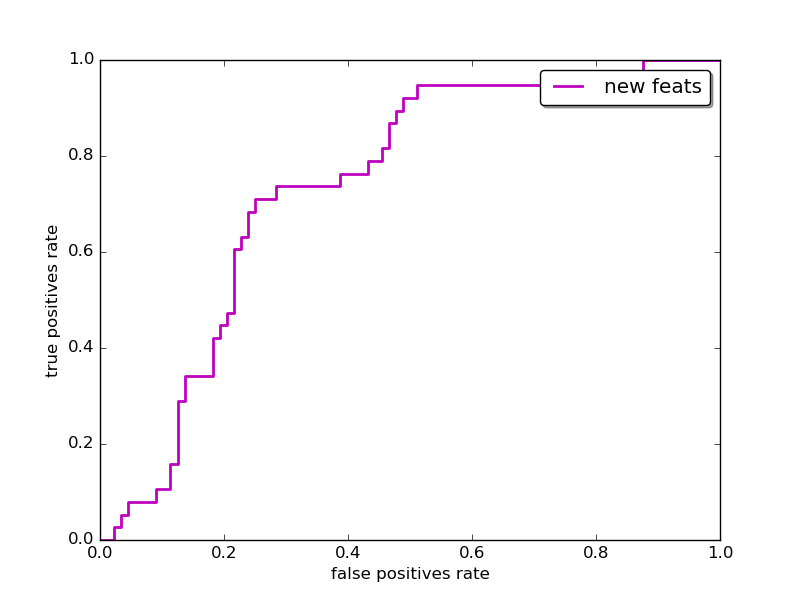
\includegraphics[width= 0.5\textwidth]{lupus_roc.png}
		%			\caption{roc curve for models of Line 5 of Table \ref{table:exp_res}.}
		\label{fig:roc_best}
	}
	\subfloat[Sensitivity-specificity curve]{
		 	\centering
		 	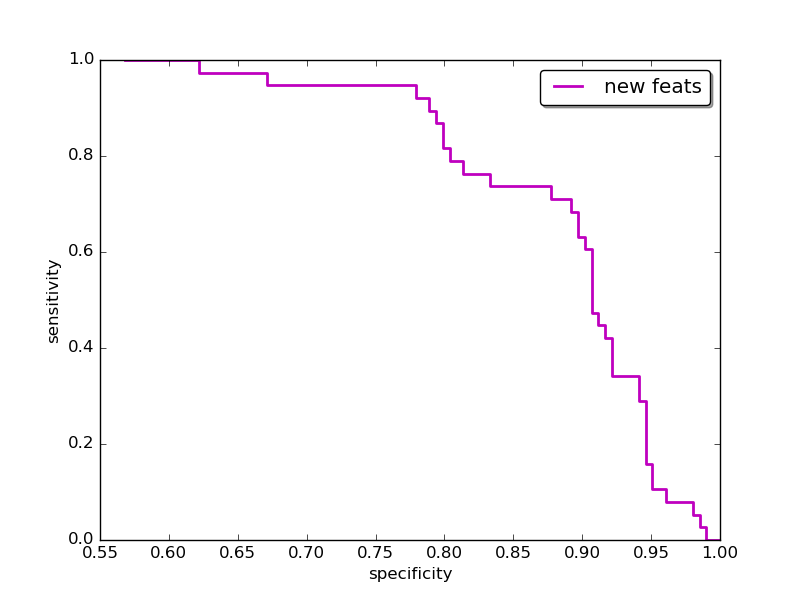
\includegraphics[width= 0.5\textwidth]{lupus_sensitivity_specificity.png}
		 	%			\caption{Sensitivity-specificity for models of Line 5 of Table \ref{table:exp_res}.}
		 	\label{fig:sensitivity_specificity_best}
	 }
\end{figure}

\end{frame}


 
